\documentclass{mcmthesis}
\mcmsetup{CTeX = false,   % if use CTeX,set this value as true
        tcn = 2118645, problem = B, %set team number and problem chosen
        sheet = true, titleinsheet = true, keywordsinsheet = true,
        titlepage = false, abstract = true}%set title page as false can delete the second summary page
\usepackage{newtxtext}
\usepackage{cleveref}

\title{Adopt Drones Distribution Model to Fight Wildfires}

\begin{document}
\begin{abstract}

Midsummer has been mild on Australia’s southeast coast, however the season was devastated by massive fires last summer. Even until next year, Australians have been under the stress and alarmed with unprecedented wildfires in especially Victoria and NSW state. Wildfires have brought devastating damage to Australia, vast areas of agriculture lands and houses were burnt, numerous wild animals were killed, massive puff of smoke they produced even circled the earth and mixed with the atmosphere. The aim of this essay is to build a Drone Distribution Model to help with monitoring fire events and giving directions to front-line personnel. We are expected to calculate the optimal number of the mix of SSA drones and radio-repeater drones that can finish the task with fire-related attributes and geographic factors taken into account, and keep the budget as low as possible. Three models are established: Model I: Hybrid Drone Routing Model;Model II: Fire Events Prediction Model; Model III: Radio-repeater Drone Distribution Model.

For Model I, fire events data from October 2019 to January 2020 of Victoria State is firstly collected. Then, as every piece of data contains longitude and latitude, their distribution on a map can be drawn.

Next, we process the data by adopting K-means clustering algorithm, thus several clusters are formed. By analyzing the attributes of fire events, we can gather information about their frequency and scale. The location and number of EOC is then determined. On consideration of the battery limit and flying range of every drone, we can determine the ratio of SSA drones and Repeaters drones. Then revise the model by setting fire scale as parameter, the optimal number of drones can be calculated.

For Model II, we randomly ganerate some clusters. After confirming the locaiton, we use some linear functions to calculate the weighted average. Then we use three kinds of fire types to distinguish the effect of different durations and simulate the date that fire occurs based on that.

Then we use Runge-Kutta and the clusters above to predicte data of the next ten years. Finally we  evaluate the model from three aspects: hit\_rate, work\_days and miss\_rate, and work out its final grade.

For Model III, we use DEM data to establish the 3D topography Model. For the repeaters, we place them at higher altitude area. To realize this process, we add altitude arguments into the grading of a pixel, so pixel with higher grade would have the probability to place repeaters. For the SSA drones, we use surface model to calculate a sphere whose  radius can make it tangent to the surface. And use surface area to replace area on 2D map by using Graham algorithm.



\begin{keywords}
UAV, repeater, wildfire, K-means, prediction model, time sequence, 3D topology model. 
\end{keywords}
\end{abstract}
\maketitle

\tableofcontents 

\section{Introduction}
\subsection{Background}
\quad \,Wildfire means uncontrolled fire in a forest, fueled by drought, heat, and wind. Since July, the second half of 2019 has witnessed burning Australia in a raging fire. The disaster was triggered by extreme drought, with strong wind and lighting adding to its intensity, it engulfed every part of the country, destroying more than 2,000 houses and forcing thousands to flee the southeastern coast under blood-red skies. The federal government has sent in military assistance for firefighting, search and rescue, and clean-up efforts, but the fire still lasted for 210 days, burning more than 17.9 million acres. A total number of 5 billion animals were killed, putting endangered species at the risk of extinction. Thick plumes of smoke have not only blanketed Australian’s urban center, but also drifted halfway around the world, threatening people’s health.

The drone would have the ability to ignite and monitor fires in remote areas. Novel technology would allow it to operate in harsh environments with limited supervision, providing a safe mechanism for people to perform fire management tasks with less risk and higher efficiency. With repeater acting as a substitute for two-way radio, the range of mutual communication is greatly extended.

\begin{figure}[h]
	\small
	\centering
	%\begin{minipage}{0.49\linewidth}
	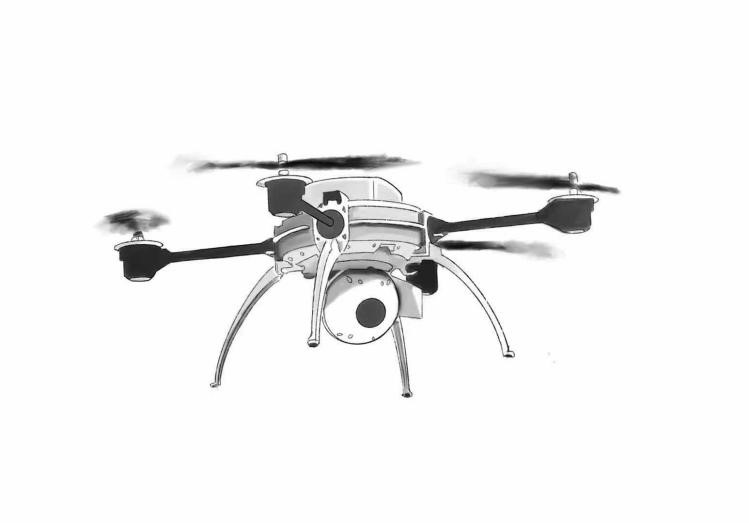
\includegraphics[width=8cm]{Figure/UAV.png}
	\caption{UAV (Unmanned Aerial Vehicle), an uncrewed aerial vehicle that can fly over combat zones and staging areas. There exist two types of UAVs in our model. 
	(a) Used for monitoring fire events and duplex communication between control center and front-line personnel.  
	(b) Carry a repeater that can rebroadcast signals with higher powers to expend the range of communication.} \label{fig:UAV}
	%\end{minipage}
\end{figure}
\subsection{Restatement of the Problem}
\begin{itemize}
	\item Build a model to calculate the optimal numbers of a mix of SSA drones and drones with repeaters that Victoria’s CFA should purchase to meet both safety and budget requirements. 
	
	\item Base upon previous data to predict the fire events in the next ten years, and evaluate the effectiveness of the model you created. View drone cost as a constant and estimate how many drones will be added if the model is to handle the worst case, causing an increase in equipment cost.
	
	\item Reconstruct the model by taking terrains and fire scale into account, and determine the locations of hovering VHF/UHF radio-repeater drones.
	
	\item With the support of your model, write an annotated Budget Request to the Victoria State Government to explain how the display of drones can help to deal with wildfires. 
\end{itemize}

\subsection{Our Approach}

\begin{itemize}
\item Build a model to calculate the optimal numbers of a mix of SSA drones and drones with repeaters that Victoria’s CFA should purchase to meet both safety and budget requirements. 

\item Base upon previous data to predict the fire events in the next ten years, and evaluate the effectiveness of the model you created. View drone cost as a constant and estimate how many drones will be added if the model is to handle the worst case, causing an increase in equipment cost.

\item Reconstruct the model by taking terrains and fire scale into account, and determine the locations of hovering VHF/UHF radio-repeater drones.

\item With the support of your model, write an annotated Budget Request to the Victoria State Government to explain how the display of drones can help to deal with wildfires. 

\end{itemize}



\section{General Assumptions, Notations and Model Overview}
\subsection{Assumptions}
To simplify the problem, we make the following basic assumptions, each of which is properly justified.
\begin{itemize}
	\item Weather condition remains the same during the analyzing process, thus we do not consider the effect of wind and heat on the fire.
	
	\item All drones fly and hover at the same height in the first model, each programmed with different routes, meaning no bumping or crushing will occur. Also, the drone itself does not break down and functions well.
	
	\item The smoke and heat produced by burning fire will not interfere with a drone’s operation: its camera lens will not be blurred, and its communication field will not be disturbed by radiation. 
	
	\item Drone control centers also function as drone charging stations. The distribution map of control centers in Victoria State is based on the frequency and scale of fire events. We see the station as a center, and the flying range of each drone is within a circle with a radius of 30km.
	
	\item There is no interference of signals between the drones, all SSA drones and drones with repeaters achieve their maximum capability. 
	
	\item According to the study of terrain, urban distribution and fire data, it is found that the bushfires of Victoria State are highly representative. Therefore, we only consider Victoria State when building all three models. 
\end{itemize}

\subsection{Notations}
The primary notations used in this paper are listed in \Cref{table:symbol} Table1.


\begin{center}
\begin{tabular}{ccc}
	\hline
	Symbol & Definition & Unit\\
	\hline
	lat & latitude of a pixel & °\\
	lon & longitude of a pixel & °\\
	C	& a cluster generated from some piexels \\
	S   & area of a cluster & ${\rm km^2}$\\
	V   & scale of a fire \\
	T   & duration of a fire & minutes \\
	MT  & the longest duration among all fire & minutes\\
	${\bf Dis_{a-b}}$ & distance between a and b & km\\
	H   & hit rate of EOCS \\
	M   & assessment result for out model \\
	\hline
	\label{table:symbol}
\end{tabular}
\end{center}
\begin{center}
	Table 1: Notations
\end{center}

\subsection{Model Overview}

\quad \, Firstly, build a Hybrid Drone Routing Model. We mark the locations of fire events and use K-means to form clusters and distinguish their intensity. 

Secondly, design a Fire Events Prediction Model. We use the historical data from October 2019 to January 2020 to predict extreme fire events in Victoria State of the next ten years. Then use the prediction result to evaluate our previous model and calculate how many drones need to be added.

Thirdly, we establish a Radio-repeater Drone Distribution Model by taking the terrain element into account. Then figure out the final cost of the whole model.

In summary , the whole modeling process can be shown as follows

Distribute drones scientifically to fight wildfires
The Australian wildfires that started from July 2019 and ended in January 2020 attracted the attention of people all around the world. Its source may be extreme drought and high temperature, then the strong wind and changeable climate made the blaze out of control. Although military force and international aid have both played a part in fire-fighting, the disaster still lasted for 210 days, causing irretrievable damage both ecologically and economically. 

As estimated, the wildfires losses exceed 100 billion AUD, and the government planned to spend over 20 billion AUD on the recovery construction. The losses increase almost exponentially as time goes by, so every single day can make a great difference. 21st century is the era of high technology, with the hottest topic being interdisciplinary products. UAV would be a good example to explain this concept if we combine its flying function with a camera that can monitor changes and a repeater that can expand communication range. The cooperation with both types of drones can ensure safety of firemen and improve fire-fighting efficiency. Here we will explain our model and show a scientific method of distributing	 drones. 

\subsection{Dataset}
\subsubsection{Data Colletcion}

\begin{center}
	\begin{tabular}{ccc}
		\hline
		Database & website & data type\\
		\hline
		Google Scholar & \url{https://scholar.google.com/} & Academic paper\\
		Kaggle & \url{https://www.kaggle.com/} &  Fire event\\
		Google map & \url{https://www.google.com/maps/} & Geography\\
		Topographic map & \url{https://topographic-map.com/} & Geography\\
		Mapbox & \url{https://studio.mapbox.com/} & Map Style\\
		Center for Disaster Philanthropy & \url{https://disasterphilanthropy.org/} & Event Report \\
		\hline
		\label{table:data}
	\end{tabular}
\end{center}
\begin{center}
	Table 2: Data Source
\end{center}
\subsubsection{Data Cleaning}
\quad \, Dataset I is fire events record of Australia from October 2019 to January 2020. For the data with ambiguous time, we predict its date on the basis of the dataset’s logical arrangement, interpolating them linearly along the time axis. As we only consider Victoria State when building models, four points are chosen to cover the state on a map. Then we filter out the data which has latitude and longitude within the range, reducing the number of data.  

\begin{figure}[h]
	\small
	\centering
	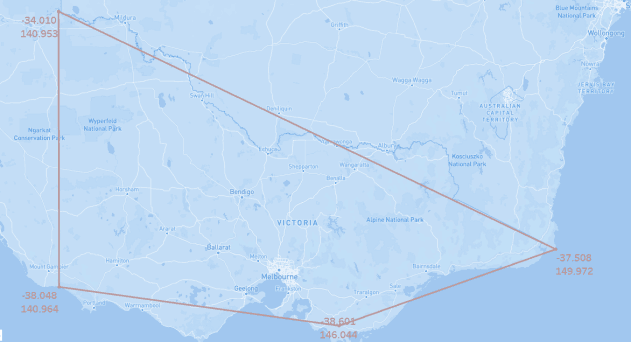
\includegraphics[width=0.8\linewidth]{Figure/Victoria.png}
	\caption{Use four points to determine the area of Victoria Stste, only data within the quadrilateral is processed.} \label{fig:Victoria}
\end{figure}

Dataset 2 is the terrain of Victoria State. The data is acquired from google map as a form of DEM. Digital Elevation Model data can reflect local terrain features with a certain resolution, thus can be used in the portrait of 3D topography model. We directly import the data into certain software and draw a 3D map that describes the terrain of Victoria State.

\section{Model I: Hybrid Drone Routing Model}
\subsection{Model Theory}
\quad \, The data of fire events we download from kaggle[1] it in the format of csv, which contains millions of data. Every piece of the data is comprised of the following attribute:
\begin{itemize}
	\item latitude: Latitude of pixel.
	\item longitude: Longitude of pixel.
	\item brightness: The temperature of the fire pixel, in Kelvin.
	\item scan: The width of the pixel at a particular location.
	\item track: The height of the pixel at a particular location.
	\item acq-date: The date the data for this pixel was acquired.
	\item acq-time: The time where the data for this pixel was acquired.
	\item satellite: Either aqua or terra.
	\item instrument: Instrument the data was collected with.
	\item confidence: Confidence of the fire at a pixel, from 0 (low-confidence of a fire) to 100 (high confidence of a fire).
	\item version: the version of this piece
	\item frp: Fire radiative power
\end{itemize}

\quad \,Every piece of data describes a pixel’s information, but it is demanding yet meaningless to analyse the pixel one by one. The locations where fires occur are marked out as points on the map, first we adopt K-means clustering algorithm to process the data. We aggregate the points that are close to each other into a cluster. Then there is another question: As the area of different clusters may be huge, we combine the cluster algorithm and recursion method. Recursive k-means will calculate a cluster’s area, if it is bigger than the threshold value that we presuppose, k-means function will operate again to split it into several smaller clusters.
The elements, including fire temperature, radiation rate, frequency, and cluster size, that describe the mountain fire are converted into an attribute vector abstractly. According to the clustering results, Victoria State is divided and the intensity of mountain fire is distinguished by color. Darker color means a more severe fire situation, and vice versa. We will discuss them in the following part. 

Finally, the number of SSA and Repeaters, the location of EOC will be calculated based on the distribution of clusters.



\subsection{Graham Algorithm}
\quad \, Our first task is to transform the discrete pixels into successive clusters, and several parameters are needed to describe a cluster. The area of a cluster is an important variable. We use k-means to acquire several clusters, but the area is still unknown because of its irregular shape. The  solution is Graham Algorithm, which can calculate dots’ minimum convex hull.\cite{gholami2019droneassisted}

We assume there is a realization of stack, and we can visit every element of the stack through repeatedly pushing and popping. stack[i] stands for the stack’s i-th element, stack.size means its size.

Polar coordinates is used to calculate the polar diameter.

\begin{equation}
		Polar Diameter = \sqrt{latitude^2+longitude^2}
\end{equation}

\begin{equation}
	Polar Angle=\left\{
	\begin{array}{rcl}
		atan(y/x) & & {x > 0 \,\,and\,\, y > 0}\\
		atan(y/x)+2pi & & {x > 0 \,\,and\,\, y < 0}\\
		atan(y/x)+pi & & {x < 0 \,\,and\,\, y < 0}\\
		atan(y/x)+pi & & {x < 0 \,\,and\,\, y > 0}
	\end{array} \right.
\end{equation}

\begin{tabular}{l}
	\hline
	Algorithm 1: Graham Algorithm \\
	\hline
	Input: some pixels called pixels[n].\\
	Output: the area of their minimum convex hull.\\
	stack s;\\
	sort pixels with latitude as first keywords \\
	for i = 1 to n do \\
	\qquad pixels[i].latitude -= pixels[0].latitude.\\
	\qquad pixels[i].longitued -= pixels[0].longitude.\\
	\qquad using equation (2) to calculate the polar diameter.\\
	\qquad using equation (3) to calculate the polar angle.\\
	sort pixels with polar angle as first keywords.\\
	push pixels[1] to pixels[3].\\
	for i = 4 to n do \\
	\qquad while s.size > 2 \\
	\qquad\qquad calculate cross product between vector(s[back-1],s[back]) and vector(s[back],s[i]) \\
	\qquad\qquad if cross product < 0 \\
	\qquad\qquad\qquad break \\
	\qquad\qquad else s.pop  \\
	answer = 0 \\
	for i = 2 to s.size \\ 
	\qquad using equation(2) to calculate val between s[i] and s[i-1] \\
	\qquad answer += val\\
	return answer \\
	\hline
\end{tabular}

Through above algorithm, we can get the area of any clusters. And it will help us a lot in the next task. \\
\subsection{Clustering Algorithm}
\quad \, As is mentioned above, we use a recursive k-means clustering algorithm to generate an array of clusters.

Before describing the algorithm, we’d like to introduce our parameters first.
\begin{itemize}
	\item node: a pixel on the map, it has follow member:
		\begin{itemize}
			\item longitude
			\item latitude
			\item brightness: The temperature of the fire pixel
			\item frp: Fire radiative power
			\item date-time: The time where the data for this pixel was acquired.
		\end{itemize}
	
	\item cluster: the product of pixel
		\begin{itemize}
			\item longitude: the average longitude of pixels it contains
			\item latitude: the average latitude of pixels it contains
			\item value: the description of the fire scale
			\item frequency: the days and frequency of this cluster
			\item area: the area of this cluster
		\end{itemize}
	
\end{itemize}

\begin{tabular}{l}
	\hline
	Algorithm 2: K-means Clustering Algorithm \\
	\hline
	Input: an array of node which called nodes, the size if about 1e5\\
	Output: an array of cluster which called clusters\\
	set a k value \\
	random k nodes to be centers.\\
	while true, do \\
	\qquad for each node, calculate the distance between node and center.\\
	\qquad then select the closest center to be its group, add this node to this group.\\
	\qquad for each center, using the average location to replace the origin location. \\
	\qquad if centers and group nolonger changed, break.\\
	for each group, record its members and average value. make cluster by the group. \\ 
	\hline
\end{tabular}

\begin{tabular}{l}
	\hline
	Algorithm 3: Rescurive K-means Clustering Algorithm \\
	\hline
	Input: an array of node which called nodes, the size if about 1e5\\
	Output: an array of cluster which called clusters\\
	using Algorithm 2 to get clusters. \\
	for each cluster: \\
	\qquad using Algorithm 1 to get its area. \\
	\qquad if the area is t0o big: \\ 
	\qquad \qquad using Algorithm 2 to process this cluster,until every of its piece is small enough. \\
	Merge all cluster to be in the same array. \\
	return this array. \\
	\hline
\end{tabular}

After using the algorithm above, we get the result as \Cref{fig:Cluster}.

\begin{figure}[h]
	\small
	\centering
	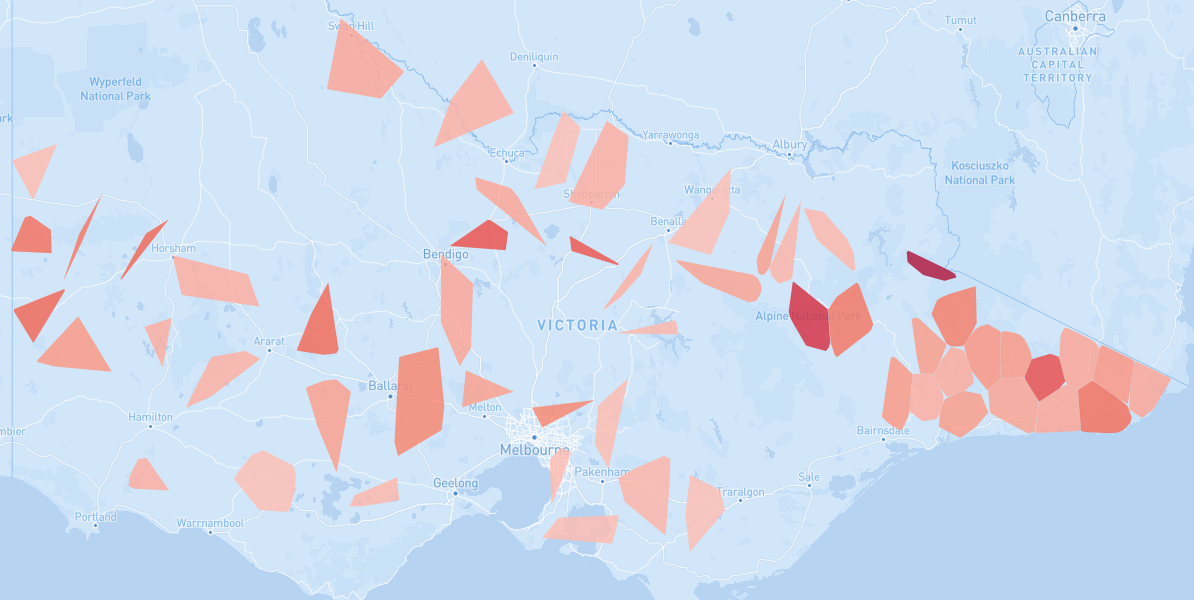
\includegraphics[width=0.7\linewidth]{Figure/Cluster.png}
	\caption{the cluster result} \label{fig:Cluster}
\end{figure}
\subsection{Location of EOC}
Next question is how to confirm the location of EOC on the basis of the thought bipartite graph and union find sets.\cite{shakhatreh2018optimal}
The ideal location of a EOC should be as close as possible to the cluster. The more numbers of clusters an EOC can reach, the better the location of EOC.

\begin{tabular}{l}
	\hline
	Algorithm 4: Dichotomy Algorithm \\
	\hline
	Input: the data of clusters\\
	Output: the location of EOC\\
	set a minv. \\
	using bipartite graph to split the map into two pieces. \\
	if two clusters are in the different piece,the distance between should bigger than minv.\\
	Make minv smaller and continue to split the map. \\
	Until the area of each piece is small enough. \\
	Then the center of the piece of map should place an EOC. \\
	Record these locations and store them into an array.\\
	return the array. \\
	\hline
\end{tabular}

\Cref{fig:EOC} show the location of EOC, the red circle is the action range.
\begin{figure}[h]
	\small
	\centering
	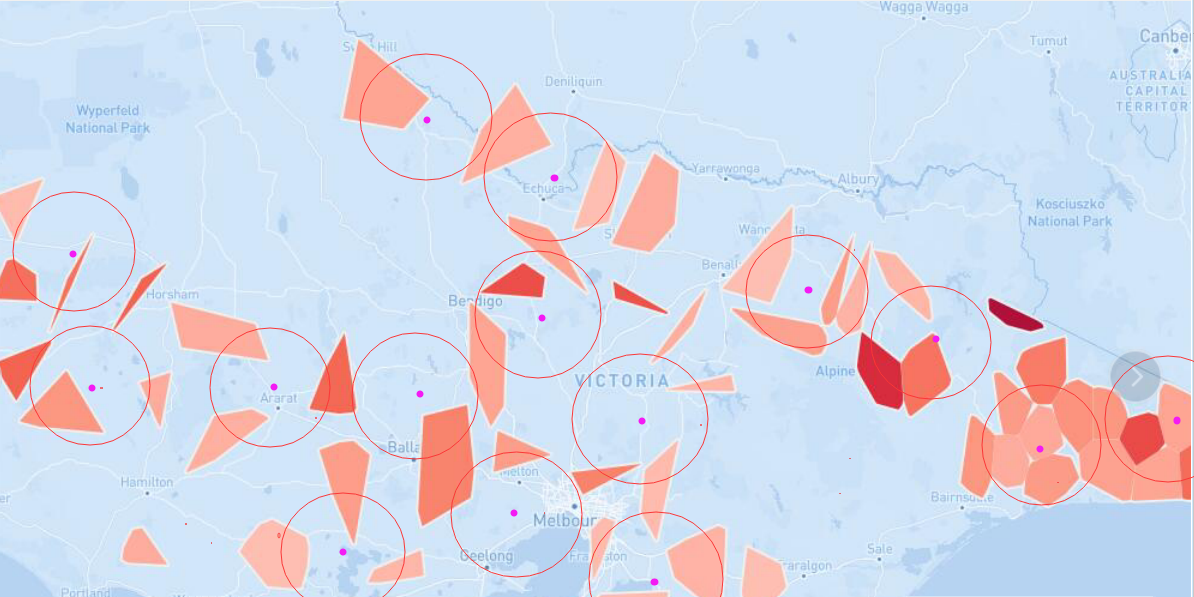
\includegraphics[width=0.8\linewidth]{Figure/EOC.png}
	\caption{the location of EOC} \label{fig:EOC}
\end{figure}
\subsection{Number of UAV}
The final problem is to arranging the number of UAV for each EOC, both SSA and Repeater.
We have below conclusions:
\begin{enumerate}
	\item As repeater is only used for expanding communication range, only one repeater is needed for each cluster.
	\item The Repeater can achieve a range of 20 km, but the action range of drone is 30km. So for drones that are further away from the EOC, we may need more than one Repeater.
	\item UAV has limited battery power, and need to recharge. By taking its speed and flying time into consideration, if the fire duration is less than 225 minutes, two SSA UAVs can finish monitoring task alternately (by taking turns), if it is larger than 225minutes, three SSA UAVs are needed.
	\item For cluster that has vast area and high intensity, we should consider this as safety claim and arrange  more SSA drones.
\end{enumerate}

So based on this, we can calculate the appropriate number of UAV.
\begin{equation}
	{\rm number\,\,of\,\,Repeater}=\left\{
	\begin{array}{rcl}
		1 & & {\rm (if\,\, all\,\, clusters\,\, are\,\, close\,\, to\,\, EOC(within\,\, 20km))}\\
		2  & & {\rm (there\,\, are\,\, at\,\, least\,\, one\,\, cluster\,\, that\,\, far \,\,from\,\, EOC)}\\
		3 & & {\rm (more\,\, than\,\, one\, \,cluster \,\,and\,\, their \,\,angle\,\, is \,\,bigger\,\, than\,\, pi/2)}\\
		4 & & {\rm (more\,\, than\, \,one\,\, cluster \,\,and \,\,their \,\,angle \,\,is \,\,bigger \,\,than \,\,3pi/2)} \\
		5 & & {\rm (four\,\, directions\,\, all\,\, have \,\,far\, \,cluster)}
	\end{array} \right.
\end{equation}

\begin{equation}
	{\rm number\,\,of\,\,SSA}=\sum_{i=1}^n {\rm (cluster_i.value*weight_1+cluster_i.area*weight_2) / base\,value}
\end{equation}

\begin{equation}
	{\rm number\,\,of\,\,UAV}=\left\{
	\begin{array}{rcl}
		{\rm number\,\,of\,\,UAV*3} & & {\rm (if\,\,fire\,\,durartion\,\,is\,\,longer\,\,than\,\,225minutes)}\\
		{\rm number\,\,of\,\,UAV*2}  & &{\rm (if\,\,fire\,\,durartion\,\,is\,\,shorter\,\,than\,\,225minutes)}\\
	\end{array} \right.
\end{equation}

Through equation(4)(5)(6),we can get the location of EOC and number of UAV, as Table 3 in \Cref{table:UAV}.

\begin{center}
	\begin{tabular}{ccccc}
		\hline
		ID & Latitude & Longitude & SSA & Repeater \\
		\hline

		1 & -37.0792 & 141.705 & 17 & 8 \\
		2 & -36.3844 & 141.453 & 6 & 6 \\
		3 & -37.2174 & 142.919 & 24 & 15 \\
		4 & -38.0103 & 143.329 & 12 & 6 \\
		5 & -37.1358 & 143.975 & 18 & 6 \\
		6 & -35.6897 & 143.959 & 12 & 6 \\
		7 & -36.1747 & 144.787 & 18 & 6 \\
		8 & -36.884 & 144.747 & 12 & 6 \\
		9 & -37.8113 & 144.582 & 6 & 6 \\
		10 & -37.3491 & 145.441 & 28 & 15 \\
		11 & -38.2026 & 145.543 & 6 & 6 \\
		12 & -36.5809 & 146.647 & 45 & 15 \\
		13 & -36.7676 & 147.478 & 39 & 15 \\
		14 & -37.379 & 148.483 & 42 & 15 \\
		15 & -37.4534 & 149.504 & 6 & 3 \\
		sum & / & /& 291 & 134 \\
		\hline
		\label{table:UAV}
	\end{tabular}
\end{center}
\begin{center}
	Table 3: Number of UAV
\end{center}

\section{Model II: Fire Events Prediction Model}
\subsection{Theoretical Basis}
\quad \, This task is divided into two parts: prediction and assessment. In the prediction part, our method combines historical data and random function to generate the predicted data. In the assessment part, we set up our own assessment model to grade the predicted data, and return some parameters which can describe the performance of Model I.

Before explaining our model, some assumptions are made to rationalize our prediction.\cite{pham2018distributed}
\begin{enumerate}
	\item We use cluster as the basic unit of prediction, rather than pixel or node.
	\item The location of cluster should be random and different every time. But if a region is closer to a cluster, the probability of it being selected is higher.
	\item The duration of a fire, the are of cluster are also random, but not completely. Based on the  previously nearby cluster, we will calcluate a base value, and the final value will float between  base value, the domain of walker should be random.
	\item The duration of a fire may be as short as one day, or as long as serval months.
	\item If a fire is put out, then within a short period, a new fire will not be started in the same region. There exists a cooling cycle to enable the plant cover to grow. The duration of cooling cycle should be relevant to the duration  of fire.
\end{enumerate}

\subsection{Random Generatation of Fire}
We should start from generating a single fire. The first argument we should confirm is location. Although location is random, two basic rules should be followed:\cite{Malandrino_2019}
\begin{itemize}
	\item the coordinate is within the range of Victoria State.(the coordinate is in Victoria.)
	\item a pixel’s selected probability should be relevant to its distance from other clusters.
\end{itemize}
if we use rand-i as a symbol of random integer, and rand-f means random float, then the latitude and longitude will be calculated as following:
\begin{equation}
	\begin{cases}
		{\rm latitude} = -34-rand\_i\%4-rand\_f; \\
		{\rm longitude} = 140+rand\_i\%10+rand\_f;\\
		{\rm longitude} > 140.952893 \\
		{\rm latitude} > -0.108776*{\rm longitude}-22.714517 \\
		{\rm latitude} > 0.278158*{\rm longitude}-79.223946 \\
		{\rm latitude} < -0.387852*{\rm longitude}+20.658908
	\end{cases}
\end{equation}

After the location is determined, we should calculate the fire’s frequency and scale. Other  cluster close to this one should take up the some proportion, the weight is inversely proportional to distance, so distance should play a role as denominator. To avoid the appearance of infinity, we need to add a laplace smoothing.
\begin{equation}
	{\rm new.area} = \sum_{i=1}^n {\rm (weight_1+rand\%limit)/(1+distance_i)*cluster_i.area}
\end{equation}
\begin{equation}
	{\rm new.scale} = \sum_{i=1}^n {\rm (weight_2+rand\%limit)/(1+distance_i)*cluster_i.scale}
\end{equation}
\begin{equation}
	{\rm new.frequency} = \sum_{i=1}^n {\rm (weight_3+rand\%limit)/(1+distance_i)*cluster_i.frequency}
\end{equation}

We can get the total fire days from frequency, but the number of fires and a fire’s duration are still not  confirmed. We define three types of fire in a simple way, respectively called big fire, midium fire and small fire. All of them have different duration and cooling cycle.
  \begin{center}
  	\begin{tabular}{ccc}
  		\hline
  		Type Name & Duration & Cooling Cycle  \\
  		\hline
  		
  		Big Fire & 15-75 days & 30-90 days\\
  		Mid Fire & 5-15 days& 10-30 days\\
  		Small Fire & 0-5 days& 0-10 days\\
  		\hline
  		\label{table:Fire Type}
  	\end{tabular}
  \end{center}
  \begin{center}
  	Table 4: Fire Type
  \end{center}
The number of each type of fire is based on frequency,  calculated through the following equations:
\begin{equation}
	{\rm bigfire} = {\rm rand\%(frequency/weight_1)+base\,\,value_1}
\end{equation}
\begin{equation}
	{\rm new.scale} = {\rm rand\%(frequency/weight_2)+base\,\,value_2}
\end{equation}
\begin{equation}
	{\rm new.frequency} = {\rm rand\%(frequency/weight_3)+base\,\,value_3}
\end{equation}
$$
		\begin{cases}
			{\rm weight_1 > weight_2 > weight_3}  \\
			{\rm base\,\,value_1 < base\,\,value_2 < base\,\,value_3}\\
			{\rm  15/5< weight_1/weight_2 < 75/15} \\
			{\rm  1< weight_2/weight_3 < 15/5} \\
		\end{cases}
$$
Choose weight and basevalue that suits the equation above, it can  produce relatively reasonable data randomly. In addition, through the random acquisition of cooling cycle, we can simulate the date of fire, which is an important evaluation criteria for model evaluation. 

\subsection{Predicted Data of the Next Ten Years}
Now we can simulate the generation of a cluster. Certain number of clusters may appear every year, so firstly we should determine the number of clusters, we can use ordinary differential equation initial-value problem algorithm to solve this problem. Also, Euler-backwards algorithm and four-stage Runge-Kutta methods are used.\cite{878915}

By using 2019-2020 data, the we can get the initial-value, it’s also easy to calculate the derivative value. calculation process is as following:\\

\begin{equation}
\begin{cases}
	y'(x) = f(x,y) \\
	y(x_0) = y_0\\
	2020 <= x < 2030 \\
\end{cases}
\end{equation}


Write the taylor expansion of $y(x+h)$ at $x$
\begin{equation}
	\begin{split}
		y(x+h)
		&=y(x)+hy'(x)+\frac{h^2}{2!}y^{(2)}(x)+...+ \frac{h^p}{p!}y^{(p)}(x)+\frac{h^{p+1}}{(p+1)!}y^{(p+1)}(x+\theta h)\\
		&=y(x)+hy'(x)+\frac{h^2}{2!}y^{(2)}(x)+...+ \frac{h^p}{p!}y^{(p)}(x)+T\\
	\end{split}
\end{equation}

We assume $0 <= \theta <= 1, T = O(h^{p+1})$
if $x = x_n$,then
\begin{equation}
y(x_{n+1})=y(x_n)+hy'(x_n)+\frac{h^2}{2!}y^{(2)}(x_n)+...+ \frac{h^p}{p!}y^{(p)}(x_n)+T_{n+1}\\
\end{equation}

if we truncation $T_{n+1}$,we can get:
\begin{equation}
	y_{n+1}=y_n+hf(x_n,y_n)+\frac{h^2}{2!}[f_x(x_n,y_n)+f_y(x_n,y_n)f(x_n,y_n)]
\end{equation}
make p = 4, we can generate the equation of four-stage Runge-Kutta.
\begin{equation}
\begin{cases}
	y_{n+1} = y_n+\frac{h}{6}(k_1+2k_2+2k_3+k_4) \\
	k_1 = f(x_n,y_n)\\
	k_2 = f(x_n+\frac{1}{2}h,y_n+\frac{1}{2}hk_1)\\
	k_3 = f(x_n+\frac{1}{2}h,y_n+\frac{1}{2}hk_2)\\
	k_4 = f(x_n+h,y_n+hk_3)
\end{cases}
\end{equation}
Plug area and number as parameters into equation(13) and use equation(17) to solve, and we can get the predicted number of cluster and total area. The result are presented in \Cref{fig:Pre}.
\begin{figure}[h]
	\small
	\centering
	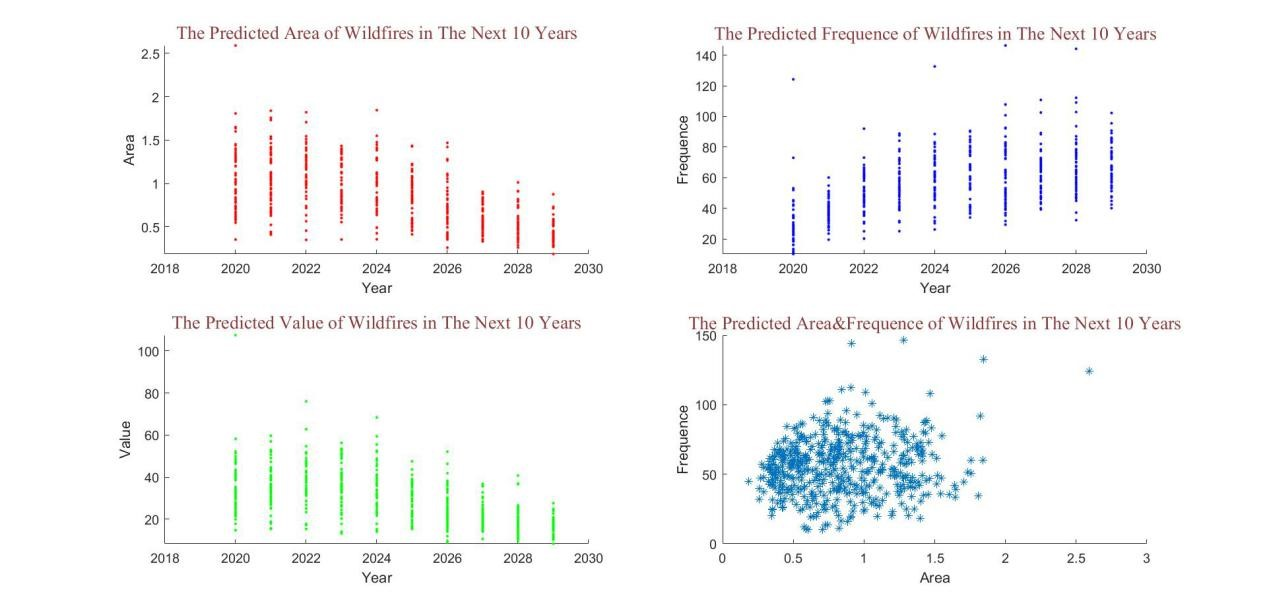
\includegraphics[width=0.8\linewidth]{Figure/Predicted.png}
	\caption{the predicted data} \label{fig:Pre}
\end{figure}

\subsection{Model Evaluation}
For the predicted fire result of each year, we use Model I to process the data, three questions should be addressed:
\begin{itemize}
	\item How many clusters can be rescued by nearby EOC?
	\item As very EOC work different days, will some be at leisure while some overwork?
	\item Does the phenomenon of lacking in UVA often occur?
\end{itemize}

We consider three parameters to be the criteria of evaluation :

\begin{equation}
	hit\_rate = hit\_times / number\_of\_clusters 
\end{equation}
\begin{equation}
	work\_rate = \sum_{i=1}^{15} work\_days_i / (15*365)
\end{equation}
\begin{equation}
	miss\_rate = miss\_days/365
\end{equation}

hit\_times means means the number of clusters that can be rescued by certain EOC.

work\_days means the number of days that EOC take action.

miss\_days means the number of days that UVA is not enough.

\begin{equation}
	Final\_Grade = 0.5*hit\_rate+0.2*work\_rate+0.3*(1-miss\_rate)
\end{equation}
All assessment result are visual in \Cref{fig:assessment}
\begin{figure}[h]
	\small
	\centering
	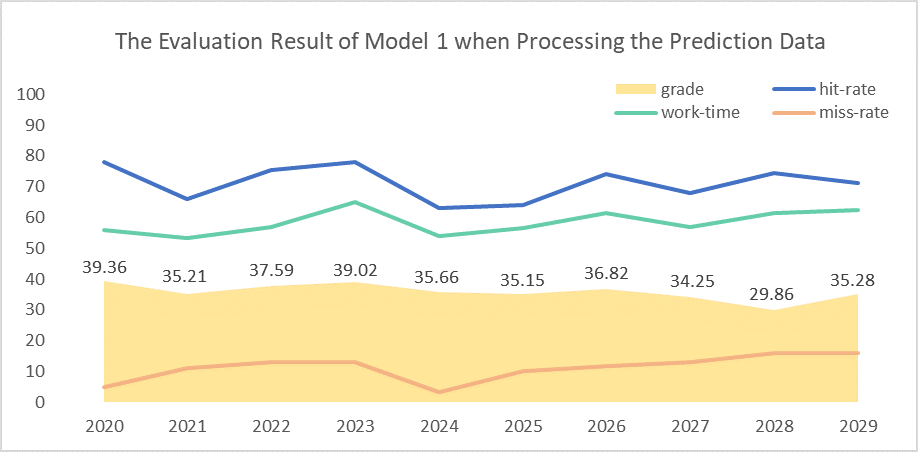
\includegraphics[width=\linewidth]{Figure/Assessment.png}
	\caption{the assessment result} \label{fig:Assessment}
\end{figure}
On consideration of extreme fire events, the optimal number of SSA drones that can complete the task is 411, so 120 drones will need to be added. The increase in its number will lead to the total expenses to rise up.
\section{Model III: Radio-repeater Drone Distribution Model}
\subsection{3D Topography Model}
In this problem, we need to consider an extra element——altitude. 
Victoria State is mainly comprised of three different landform: plain, plateau, and mountain. According to the requirements, we need to take the effect of different terrains into consideration. Therefore a 3D model that describes Victoria’s topography and a more complex distribution strategy are needed.

Due to the high altitude areas need to use another optimization of VHF repeater infinite unmanned aerial vehicle (uav), and the Australian state of Victoria mountain does not see more, so only in the jurisdiction area is arranged in the mountain of EOC optimization of VHF/UHF infinite repeater unmanned aerial vehicle (uav).

According to the survey, the elevation of mountain does not disturb a repeater’s signal, As VHF has a longer wavelength than UHF, meaning a better diffraction ability. Thus when in high altitude areas, we use only VHF radio-repeater drones. In low altitude areas, UHF radio-repeater drones are preferred. In medium altitude areas, both radio-repeater drones work together to finish the task. By adding new conditions and parameters and considering different terrains and fire scale, we can build a radio-repeater drone distribution model.
\\

In the mountainous area, we place a VHF repeater drone on the mountain-top to fully utilize its capability.


\begin{figure}[h]
	\small
	\centering
	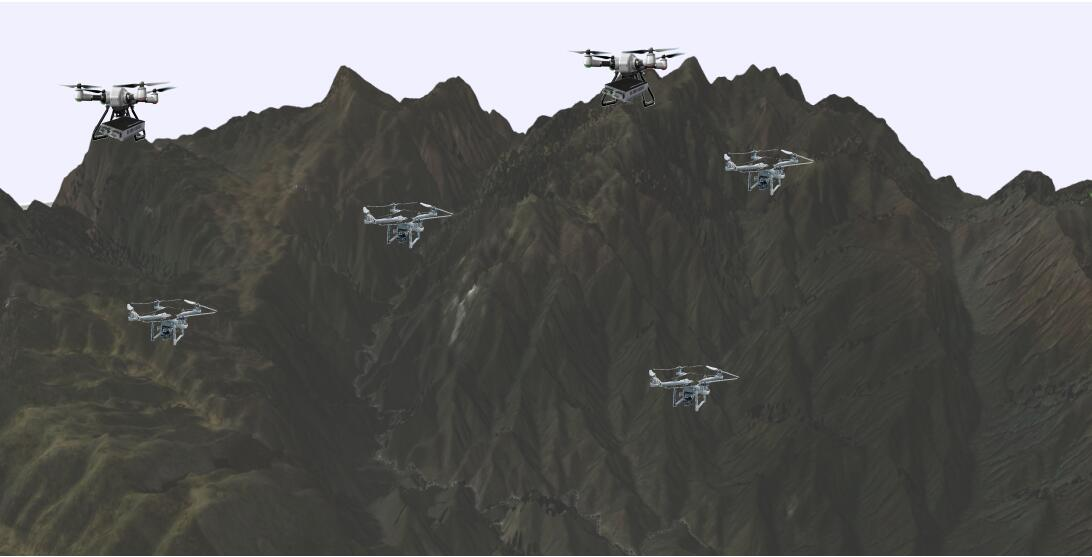
\includegraphics[width=0.6\linewidth]{Figure/3D-Model.png}
	\caption{model of distribution on 3D map} \label{fig:3D-Model}
\end{figure}
\subsection{Location of Repeater Drones}
It’s obvious that both Repeaters Drone and SSA Drone need to be rearranged, but the situation for them is a little different, so we will discuss the difference.
The task for Repeater is mainly forwarding signal, as it arrives at the destination,it probably will not  move anymore. So the power dissipation of it will not change a lot. Although its working range may be smaller, it has little effect on Repeater.
Scientists reveal that Repeater perform much better at higher altitudes than plain. We should place Repeaters on some place that both close to cluster and high attitude area. That means the grade of location should be higher as it’s on the mountain. 
In Model-I we use Dichotomy Algorithm to calculate the location of EOC, now we write an improved algorithm on the basis of it that considers altitude.


\begin{tabular}{l}
	\hline
	Algorithm 5: Improved Dichotomy Algorithm \\
	\hline
	Input: the data of clusters\\
	Output: the location of Repeater\\
	Using Algorithm 4:Dichotomy Algorithm to get splited map.\\
	Now we don't use center to be the place of Repeaters.\\
	$distance = \sqrt{(latitude-center.latitude)^2+(longitude-center.longitude)^2}$\\
	$grade = weight_1*distance+weight_2*altitude$\\
	sort all grades and select the highest grade to the target.\\
	Record these locations and store them into an array.\\
	return the array. \\
	\hline
\end{tabular}
\subsection{Rearrangement of SSA Drones}
As for SSA drones, its action range should reduce because of altitude, so we should reconsider two aspects:
\begin{itemize}
	\item Reduce the radius of circle in \Cref{fig:EOC}, and rerun Algorithm 4:Dichotomy Algorithm.
	\item Find a way to calculate the area of a curved surface.
\end{itemize}

For the new radius, we download a DEM\cite{568581} data which contains Victoria State’s altitude and base on that establish a 3D  topography Model. Use greedy thought, set lef t = 0,right =  30KM, use dichotomy to find the value which is tangent to the surface. Use this value  as radius. It’s evident that a ball whose radius is equal to this value can be contained in this  surface, so the SSA will certainly be within the range.
As for the calculation of curved surface, we use surface area formula directly:

\begin{equation}
S = \iint_{D_{yz}} \sqrt{1+{(\frac{\partial x}{\partial y})}^2+{(\frac{\partial y}{\partial z })}^2} \, dydz
\end{equation}

\subsection{Display of Optimized Distribution}
\begin{center}
	\begin{tabular}{ccccc}
		\hline
		ID & Latitude & Longitude & SSA & Repeater \\
		\hline
		
		1 & -33.1692 & 145.105 & 13 & 11 \\
		2 & -36.3844 & 141.143 & 25 & 9 \\
		3 & -34.2354 & 146.429 & 17 & 12 \\
		4 & -38.0913 & 142.082 & 21 & 8 \\
		5 & -35.8922 & 148.163 & 25 & 11 \\
		6 & -34.21i3 & 148.001 & 16 & 6 \\
		7 & -36.2104 & 143.762 & 31 & 13 \\
		8 & -35.7133 & 144.521 & 26 & 16 \\
		9 & -36.5143 & 142.127 & 19 & 11 \\
		10 & -37.3219 & 143.346 & 21 & 8 \\
		11 & -38.3951 & 144.721 & 55 & 17 \\
		12 & -35.2109 & 149.213 & 32 & 23 \\
		13 & -36.7676 & 142.062 & 28 & 10 \\
		14 & -34.2479 & 148.698 & 38 & 16 \\
		15 & -35.3512 & 141.213 & 19 & 8 \\
		sum & / & /& 387 & 179 \\
		\hline
		\label{table:3D}
	\end{tabular}
\end{center}
\begin{center}
	Table 5: Display of Optimized Distribution
\end{center}

\section{Conclusion}
\subsection{Strength}
The routing model consider the scale and frequency of fire events, prioritizing the safety of firemen to work out the distribution of SSA drones and repeater drones. Also, as the electric power of a drone is limited, charging station should be built evenly in the state. The model consider this realistic restriction, and calculate the maximum time a drone can use for working.  

The best ratio of SSA drones to repeater drones is always calculated, ensuring full coverage of fire area and stable communication between EOC and front-line personnel, at the same time using the least number of drones to cut back on the expenses.

The prediction model considers fire scale, duration time and fire sizes, describing a fire with three parameters, making the model strict in logic and inclusive in analysis. When using the prediction data to evaluate the previous model, hit-rate, miss-rate and EOC work-days are calculated through weight function to achieve the final grade. 

\subsection{Possible Improvements}
The prediction of fire events can be more accurate if we have data of a longer period, instead of data of merely 4 months;

The climate condition, including wind and temperature, should have effect on wildfires, thus a simulation model of fire need to be built on the basis of these factors.  

In real-life situations, multiple repeaters working together would produce strong interference, making each unable to fully utilize its capability. Also, as repeater has limited bandwidth, the drones that depend on it to transmit data and image must share its bandwidth. So the number of drones that a repeater can support is very disappointing. However, a new type of drone called McVision monitor use IP signals and wireless Ad-Hoc networks, that can support considerable number of drones and transmit data within millisecond.

According to basic economic laws, the price of drone will not remain constant over time. So the inflation(deflation) rate should be included in the math equation to calculate the current price of drone. Also, the cost of raw material, development of technology, trend of the whole drone industry, etc. are all complex factors that can affect its price. 

\section{Discussion}
\subsection{Real-life Scenarios}
The wildfires that happened in Australia from 2019 to 2020 have aroused global concern, a disaster of such long duration and vast area brought people deep pain. As meteorologists indicate, the global temperature has been climbing since the beginning of the century, as a result of the rapid development of technology. The burning of coal for heat and power have caused the carbon dioxide to enter the atmosphere, further lead to the melting of glacier and more severe extreme weather phenomenon. Drought is also the perpetrator of wildfire, so it is fair to predict that fires will occur more frequently in the future.

The technology always develop with the era, it is demand and utilization that give birth to even more advanced technology products. There are always reports about real-life applications of drones on Science News Website. Whether it is monitoring natural disasters or catching criminals at large, whether it is reinforcing military deployment or maintaining public order, drone can act as perfect helper under various scenarios.

\subsection{Suggestion}
The drone distribution system we put forward in this essay is a combination of SSA drones and repeater drones. SSA drones have the ability of flying to dangerous areas that humans can not enter and monitor the situation on site. For example, when there is a very serious fire disaster in a certain area, the EOC should first send out drones to capture pictures of the region and presume the fire level from the information that images present. Once the fire becomes weaker to a certain state and humans beings are safe to enter the region, fire-fighters are deployed to put out the fire. The other type of drone carries a repeater with itself, it is given another function, that is to expand the range of communication. Because of the limited signal range of two-way radio, drones are trapped in a small circle and have to be close to its control center. But with the aid of repeater, not only are the images transmitted with higher resolution and faster speed, but also can the drones fly further away to perform its task. 

Imagine if the system is widely adopted in real-life, SSA drones can send back data soon after the disaster happens, and fly back and forth numerous times to inform the latest situation, helping the rescue center to make rapid and rational decisions. In addition, the safety of fire-fighters are placed at the first place, reducing the probability of injury and death to a minimum. Apart from the two kinds of drones we mentioned above, there are other drones with special functions, such as the one that carries liquid to put out fire, and the one that equips special camera to form infrared images, etc. Therefore, it is certain to say that drones will play a greater role in the process of fighting wildfires and other disasters, and a suggestion of adopting drones in disaster prevention and addressing process is presented.


\section{newtitle}
\begin{appendices}

\section{Budget Request}

Problem Background: The Australian wildfires that started from July 2019 and ended in January 2020 attracted the attention of people all around the world. Its may be started because of extreme drought and high temperature, then the strong wind and changeable climate made the blaze out of control. Although military force and international aid have both played a part in fire-fighting, the disaster still lasted for 210 days, causing irretrievable damage both ecologically and economically. As estimated, the wildfires losses exceed 100 billion AUD, and the government planned to spend over 20 billion AUD on the recovery construction. In addition, many fire-fighters lost their lives when performing rescue and extinguishment tasks. The losses increase almost exponentially as time goes by, so every single day can make a great difference. 

Project Introduction: 21st century is the era of high technology, with the hottest topic being interdisciplinary products. UAV would be a good example to explain this concept if we combine its flying function with a camera that can monitor changes and a repeater that can expand communication range. A research project has built a drone distribution model using both types of drones to ensure safety of firemen and improve fire-fighting efficiency. The project has learned from the experience of previous research, and manage to build their own model. The project group started from gaining knowledge about related hardware and equipment, benchmarking all the products in the drone market and finally decided on the Wile-15.2X drone\cite{7989656}, which has a long battery life and outstanding anti-interference ability. The repeater they chose can expand the communication range to 20km, no matter in urban area or the countryside. Then they stimulate a 3D topography model to study the terrain of Victoria State, of which the altitude difference is quite large. Then they mark out the                 location that once had a fire between October 2019 and January 2020, analyzing the data of fire events to obtain the property of each fire. Finally the drone distribution model is established by taking terrain and fire intensity into account. The model has also been through several tests of extreme fire events, and has been revised and optimized several times to  reach the final state. 
\begin{center}
	\begin{tabular}{cccc}
		\hline
		Budget Item         &    Cost Per Item         &    Quantity &         Total Cost  \\
		\hline
		
		SSA Drone          &     10,000 AUD          &      580         &   5,800,000        \\
		Repeater Drone    &       10,000 AUD      &          270      &       2,700,000\\
		SD card            &       32 AUD       &           800       &      25,600\\
		Camera             &      500 ADD        &         300        &     150,000\\
		Camera Lens        &       50 AUD        &          250       &      12,500\\
		Charging Station   &        20,0000 AUD   &            6       &       1,2000,000\\
		&&&Total 20,688,100 \\
		\hline
		\label{table:CFA REQUEST}
	\end{tabular}
\end{center}
\begin{center}
	Table : CFA REQUEST
\end{center}






Justification:
\begin{enumerate}
	\item SSA drone is used for monitoring fire events and capturing images on site. The optimal number is 387, and we purchase 1.5 times of its optimal number.
	\item Repeater drone is use for expanding range of signal transmission. The optimal number is 179, and we purchase 1.5 times of its optimal number.
	\item Consider that sometimes drones do not function well, more drones should be bought in case of emergency.
	\item  The storage capacity of a SD card is limited, so additional MicroSD card with a capacity of 128GB should be stored in the warehouse.
	\item  The camera of a drone may be destroyed by extreme climate condition, so we need extra cameras for replacement.
	\item  Different Camera lens can help a camera take different types of pictures, so all types of lens should be purchased in order to perform special tasks. 
	\item  A charger that can power 3 batteries cost 20 AUD, one drone contains one battery, that is 7 AUD for a drone. Suppose each station can hold 100 drones, we need 6 charging stations.
\end{enumerate}



The distribution system is strict in logic and inclusive in analysis, the number of all equipment listed in the table is the optimal one. Wildfires in 2019 and 2020 caused great damage to Victoria state and the country, to prevent such thing from happening again, a more scientific way of utilizing the drones should be adopted. The expenses spent on purchasing drones and relevant equipment should be minor compared to the loss that the country have been through. Many other countries have used similar system to prevent and help with fire-fighting, and has achieved surprising result. We believe in the power of nature, that it can bring us inexhaustible resources and at the same time destroy everything we cherish. We should also have faith in the power of technology, that the wisdom of human will eventually guide us to a bright future.  



\section{References}
\bibliographystyle{plain}
\bibliography{Reference}



\end{appendices}
\end{document}
